\documentclass[12pt,a4paper]{article}
\usepackage{graphicx}
\usepackage{amsmath}
\usepackage{amssymb}
\usepackage[colorlinks=true, allcolors=blue]{hyperref}
\usepackage{url}
\usepackage[style=apa, backend=biber]{biblatex}
\usepackage[german]{babel}

% \usepackage{helvet}
% \renewcommand{\familydefault}{\sfdefault}

\usepackage[left=3cm,top=3cm,right=3cm,bottom=3cm,bindingoffset=0.5cm]{geometry}
\renewcommand{\baselinestretch}{1.5} 

\addbibresource{references.bib}

\title{Musterlösung Kurvendiskussion einer Funktionsschar}
\author{Danilo Stojanovic, Tim Gabrikowski}
\date{\today}

\begin{document}

\maketitle

\begin{abstract}
In diesem Dokument wird eine Kurvendiskussion an einer Funktionsschar durchgeführt. 
\end{abstract}

\newpage

\section{Funktionsschar}

Die zu Analysierende Funktionsschar ist die Folgende:

$$
\begin{aligned}
    f_k(x)&=(x-k)^2+\frac{k}{2} \\ 
    &= x^2 - 2kx + k^2 + \frac{k}{2}
\end{aligned}
$$

\section{Kurvendiskussion}

\subsection{Definitionsbereich}

Es handelt sich bei der Funktionsschar um eine ganzrationale Funktion 2. Grades, also ist der Definitionsbereich die Menge der reelen Zahlen.

$$
D_{f_k} = \mathbb{R}
$$

\subsection{Grenzverhalten}

Da es sich um eine Funktion 2. Grades, also graden Grades handelt kommt diese aus dem unendlichen und verläuft in die gleiche Richtung ins unendliche. Vor dem $x^2$ steht ein positiver Faktor ($1$), also kommt die Funktion aus dem positiv unendlichen und verläuft ins positiv unendliche.

$$
\lim_{x \to \pm \infty} f_k(x) = + \infty
$$

\subsection{Y-Achsenschnittpunkt}

Den Schnittpunkt mit der Y-Achse berechnet man, indem man $x=0$ in die Funktionsschar einsetzt. 

$$
\begin{aligned}
    f_k(x)&= x^2 - 2kx + k^2 + \frac{k}{2} \\
    f_k(0)&= 0^2 - 2k \cdot 0 + k^2 + \frac{k}{2} \\
    &= k^2 + \frac{k}{2} \\
\end{aligned}
$$

Daraus folgt, dass der Schnittpunkt mit der y-Achse der folgende ist:

$$
\label{eq:spy}
SP_y(0 \mid k^2 + \frac{k}{2})
$$

\subsection {Nullstellen}

Zum Berechnen der Nullstellen einer Funktion setzen wir die Funktion gleich 0 und lösen nach $x$ auf.

$$
\begin{aligned}
    f_k(x)&= x^2 - 2kx + k^2 + \frac{k}{2} \overset{!}{=} 0 \\
    x_{1,2} &= -\frac{-2k}{2} \pm \sqrt{(\frac{-2k}{2})^2 - (k^2 + \frac{k}{2})} \\
    &= k \pm \sqrt{k^2 - k^2 - \frac{k}{2}} \\
    &= k \pm \sqrt{- \frac{k}{2}} \\
\end{aligned}
$$

Wir sehen, dass auch die Nullstellen von $k$ abhängig sind.

\subsubsection{Fall 1: Keine Nullstellen}

Dieser Fall tritt ein, wenn die Gleichung 

$$ x_{1,2} = k \pm \sqrt {-\frac{k}{2}} $$

keine Lösung (in der Menge der Reelen Zahlen) besitzt. Wir sehen, dass dies der Fall ist, wenn

$$ -\frac{k}{2} < 0 $$

gilt. Wir lösen die Ungleichung nach k auf:

$$ 
\begin{aligned}
    -\frac k 2 & < 0 & \mid \cdot (-2) \\
    k & > 0 
\end{aligned}
$$

Die Kurvenschar besitzt demnach keine Nullstellen, wenn $k>0$ gilt.

\subsubsection{Fall 2: 2 Nullstellen}


Dieser Fall tritt ein, wenn die Gleichung 

$$ x_{1,2} = k \pm \sqrt {-\frac k 2} $$

2 Lösungen (in der Menge der Reelen Zahlen) besitzt. Wir sehen, dass dies nur möglich sein kann, wenn $\sqrt {-\frac k 2} \neq 0 $ gilt, da dieser Term entweder addiert, oder subtrahiert wird.

Wir lösen nun diese Ungleichung nach k auf:

$$
\begin{aligned}
    \sqrt{-\frac{k}{2}} & \neq 0 & \mid \> ()^2 \\
    - \frac{k}{2} & \neq 0 & \mid \cdot (-2) \\
    k & \neq 0
\end{aligned}
$$

Wir sehen nun, dass die Kurvenschar 2 Nullstellen besitzen kann, wenn $$k\neq 0$$ gilt. Da wir aber bereits in Fall 1 gesehen haben, dass bei $$k > 0$$ keine Nullstellen existieren, besitzt die Kurvenschar 2 Nullstellen, wenn $$k < 0$$ gilt.

\subsubsection{Fall 3: 1 Nullstelle}

Dieser Fall tritt ein, wenn die Gleichung 

$$  x_{1,2} = k \pm \sqrt {-\frac k 2} $$

1 Lösung (in der Menge der Reelen Zahlen) besitzt. Wir sehen, dass dies der Fall ist, wenn

$$ \sqrt {-\frac k 2} = 0 $$

gilt. Wir lösen die Gleichung also nach k auf:

$$
\begin{aligned}
    \sqrt{-\frac{k}{2}} & = 0 & \mid \> ()^2 \\
    - \frac{k}{2} & = 0 & \mid \cdot (-2) \\
    k & = 0
\end{aligned}
$$

Einzig die Funktion $f_0(x)$ besitzt genau eine Nullstelle. Diese befindet sich im Punkt $(0 \mid 0)$ 

\subsection{Extremstellen}

Wir bilden die Erste Ableitung der Funktionsschar. Wichtig ist, dass wir nach $x$ ableiten und $k$ wie eine Konstante behandeln:

$$
\begin{aligned}
    f_k(x) &= x^2 - 2kx + k^2 + \frac{k}{2} \\
    f'_k(x) &= 2x - 2k
\end{aligned}
$$

Wir bestimmen nun die Nullstellen der ersten Ableitung. Diese sind unsere Extremstellen.

$$
\begin{aligned}
    f'_k(x) &= 2x - 2k = 0 \\
    2x - 2k &= 0 &|\; + 2k \\
    2x &= 2k &| \; :2 \\
    x &= k
\end{aligned}
$$

Die Funktionen der Funktionen der Funktionsschar besitzen also ihre Extremstellen bei $x = k$. Wir können nun die Extrempunkte berechnen, indem wir in $f_k(x)$ für $x$ einfach $k$ einsetzen und dies Umformen.

$$
\begin{aligned}
    f_k(x)&= x^2 - 2kx + k^2 + \frac{k}{2} \\
    f_k(k)&= k^2 - 2k^2 + k^2 + \frac{k}{2} \\
    f_k(k)&= \frac{k}{2} \\
\end{aligned}
$$

Die Extrempunkte sind also $Ep_f(k \mid \frac{k}{2})$.

\subsection{Wendestellen}

Wendestellen liegen auf den Nullstellen der zweiten Ableitung:

$$
\begin{aligned}
    f'_k(x) &= 2x - 2k \\
    f''_k(x) &= 2 \overset{!}{=} 0 \\
    2 \ne 0
\end{aligned}
$$

Da diese Gleichung keine Lösung in der Menge der reelen Zahlen besitzt, besitzt keine Funktion der Funktionsschar einen Wendepunkt.

\subsection {Wertebereich}

Wir setzen hierzu die Extremstellen in die 2. Ableitung ein und sehen, dass $f''_k(x) = 2 > 0$ ist. Wir sehen, dass es sich immer um Tiefpunkte handelt. Da es eine Parabel ist, welche nur einen Extrempunkt hat, lässt sich sagen, dass die Funktion keinen Funktionswert besitzt, der kleiner als der Funktionswert des Tiefpunkts ist. Daraus folgt der Wertebereich:

$$
W_{f_k} = \{ y \in \mathbb{R}^{\ge\frac{k}{2}} : y = f_k(x), x \in D_{f_k} \}
$$

\section{Zeichnung der Funktionsschar}

Abbildung \ref{fig:draw} zeigt die Funktionsschar für  $k \in [-3, 3]_{\mathbb{Z}}$

\begin{figure}[h]
    \centering
    % \includegraphics{example-image-a}
    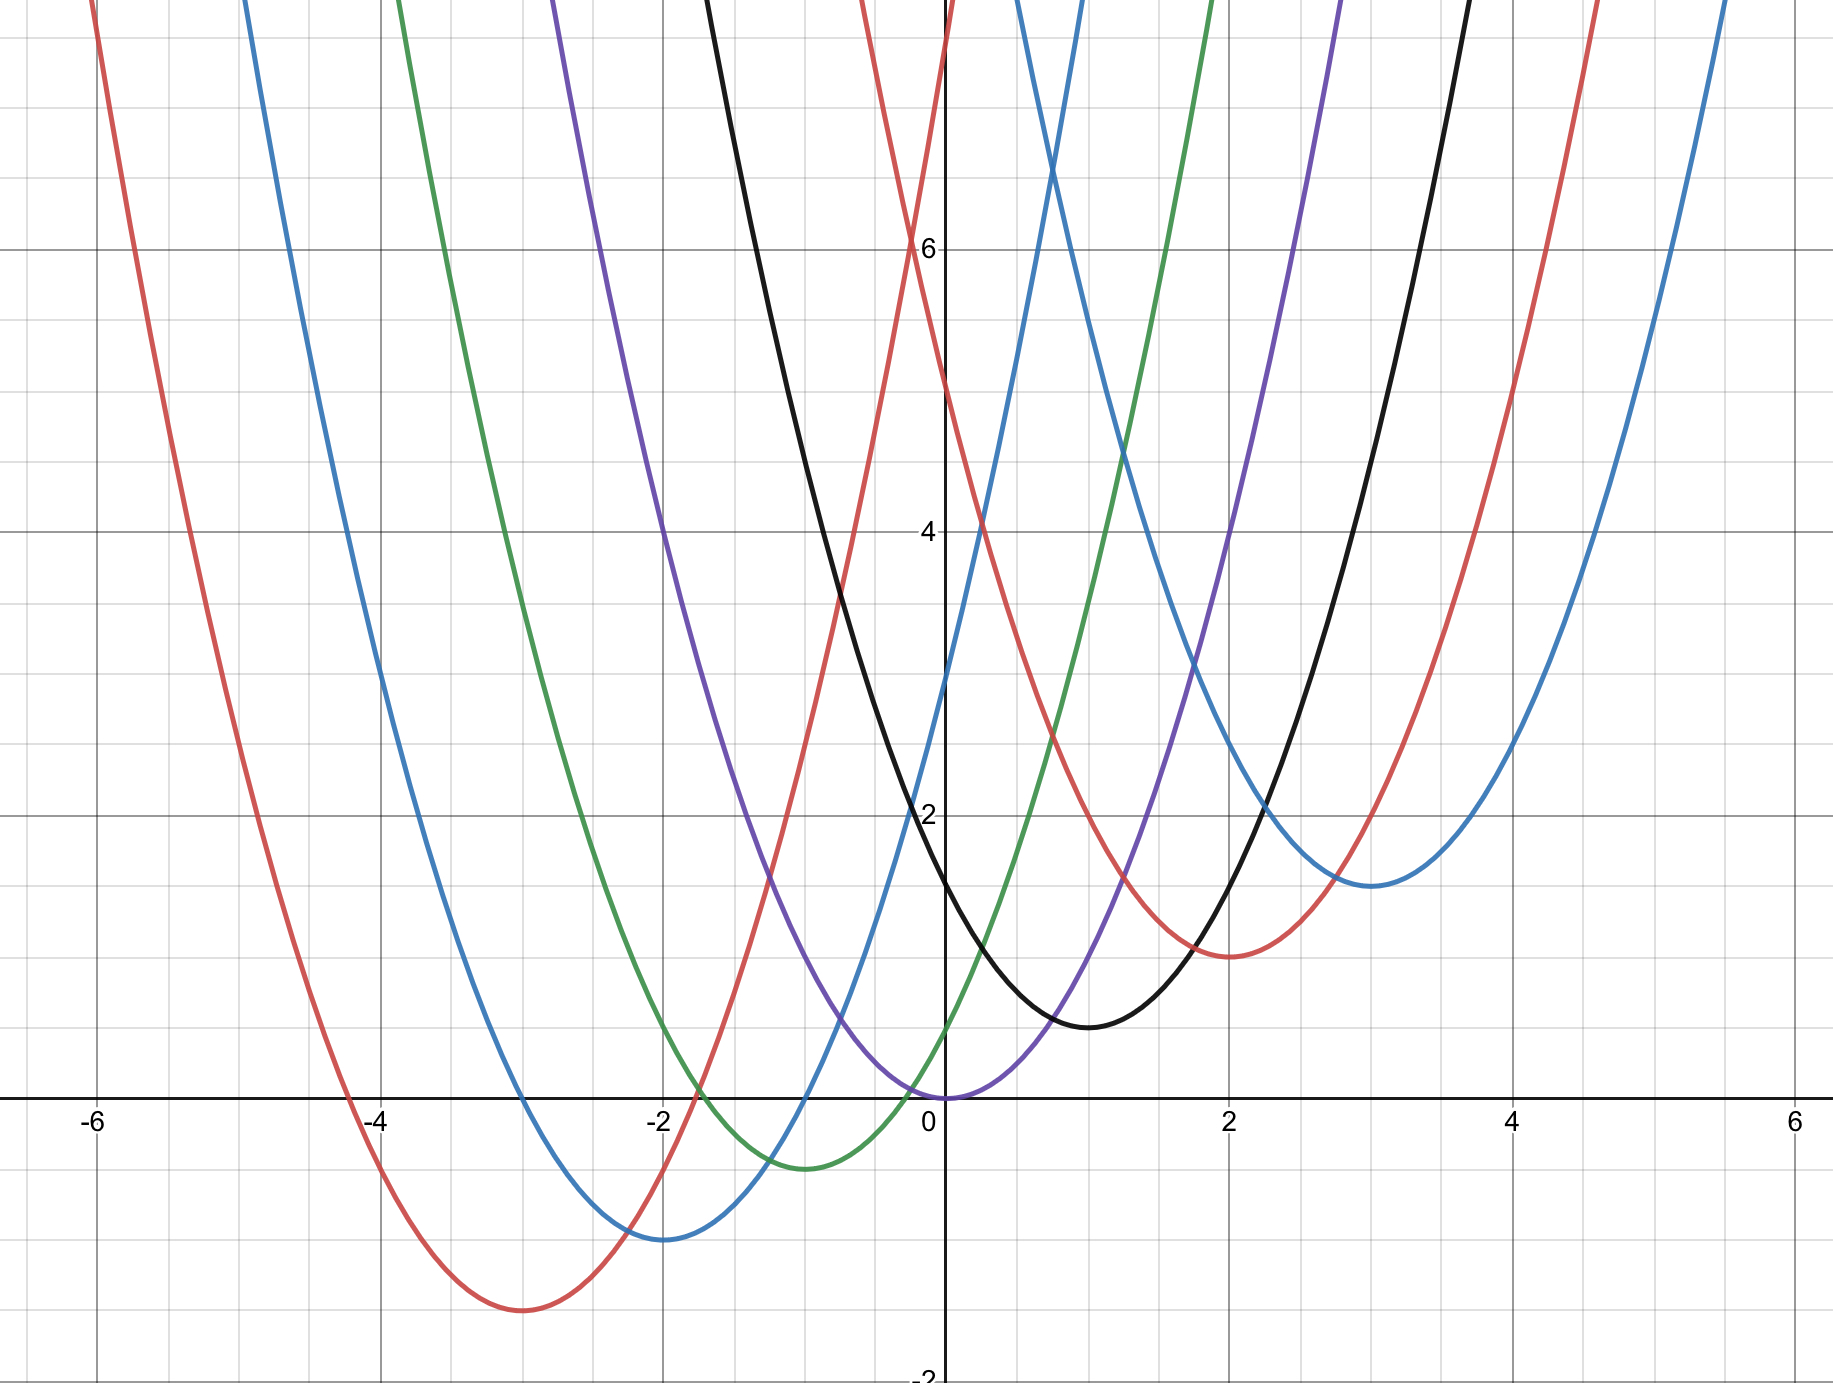
\includegraphics[width=1\textwidth]{./images/IMG_1615.jpg}
    \caption{Skizze der Funktionsschar}
    \label{fig:draw}
\end{figure}


\printbibliography[title={Literaturverzeichnis}]

\end{document}

